\documentclass[floatsintext,man]{apa6}

\usepackage{amssymb,amsmath}
\usepackage{ifxetex,ifluatex}
\usepackage{fixltx2e} % provides \textsubscript
\ifnum 0\ifxetex 1\fi\ifluatex 1\fi=0 % if pdftex
  \usepackage[T1]{fontenc}
  \usepackage[utf8]{inputenc}
\else % if luatex or xelatex
  \ifxetex
    \usepackage{mathspec}
    \usepackage{xltxtra,xunicode}
  \else
    \usepackage{fontspec}
  \fi
  \defaultfontfeatures{Mapping=tex-text,Scale=MatchLowercase}
  \newcommand{\euro}{€}
\fi
% use upquote if available, for straight quotes in verbatim environments
\IfFileExists{upquote.sty}{\usepackage{upquote}}{}
% use microtype if available
\IfFileExists{microtype.sty}{\usepackage{microtype}}{}

% Table formatting
\usepackage{longtable, booktabs}
\usepackage{lscape}
% \usepackage[counterclockwise]{rotating}   % Landscape page setup for large tables
\usepackage{multirow}		% Table styling
\usepackage{tabularx}		% Control Column width
\usepackage[flushleft]{threeparttable}	% Allows for three part tables with a specified notes section
\usepackage{threeparttablex}            % Lets threeparttable work with longtable

% Create new environments so endfloat can handle them
% \newenvironment{ltable}
%   {\begin{landscape}\begin{center}\begin{threeparttable}}
%   {\end{threeparttable}\end{center}\end{landscape}}

\newenvironment{lltable}
  {\begin{landscape}\begin{center}\begin{ThreePartTable}}
  {\end{ThreePartTable}\end{center}\end{landscape}}




% The following enables adjusting longtable caption width to table width
% Solution found at http://golatex.de/longtable-mit-caption-so-breit-wie-die-tabelle-t15767.html
\makeatletter
\newcommand\LastLTentrywidth{1em}
\newlength\longtablewidth
\setlength{\longtablewidth}{1in}
\newcommand\getlongtablewidth{%
 \begingroup
  \ifcsname LT@\roman{LT@tables}\endcsname
  \global\longtablewidth=0pt
  \renewcommand\LT@entry[2]{\global\advance\longtablewidth by ##2\relax\gdef\LastLTentrywidth{##2}}%
  \@nameuse{LT@\roman{LT@tables}}%
  \fi
\endgroup}


\ifxetex
  \usepackage[setpagesize=false, % page size defined by xetex
              unicode=false, % unicode breaks when used with xetex
              xetex]{hyperref}
\else
  \usepackage[unicode=true]{hyperref}
\fi
\hypersetup{breaklinks=true,
            pdfauthor={},
            pdftitle={Final Exam Project Report : Predict 413},
            colorlinks=true,
            citecolor=blue,
            urlcolor=blue,
            linkcolor=black,
            pdfborder={0 0 0}}
\urlstyle{same}  % don't use monospace font for urls

\setlength{\parindent}{0pt}
%\setlength{\parskip}{0pt plus 0pt minus 0pt}

\setlength{\emergencystretch}{3em}  % prevent overfull lines


% Manuscript styling
\captionsetup{font=singlespacing,justification=justified}
\usepackage{csquotes}
\usepackage{upgreek}



\usepackage{tikz} % Variable definition to generate author note

% fix for \tightlist problem in pandoc 1.14
\providecommand{\tightlist}{%
  \setlength{\itemsep}{0pt}\setlength{\parskip}{0pt}}

% Essential manuscript parts
  \title{Final Exam Project Report : Predict 413}

  \shorttitle{Jun 10 2018}


  \author{Rahul Sangole\textsuperscript{1}}

  % \def\affdep{{""}}%
  % \def\affcity{{""}}%

  \affiliation{
    \vspace{0.5cm}
          \textsuperscript{1} Northwestern University  }



  \abstract{This reports the work done for the Predict 413 Section 55 final project
assignment, Summer 2018.}
  



  \raggedbottom

\usepackage{amsthm}
\newtheorem{theorem}{Theorem}[section]
\newtheorem{lemma}{Lemma}[section]
\theoremstyle{definition}
\newtheorem{definition}{Definition}[section]
\newtheorem{corollary}{Corollary}[section]
\newtheorem{proposition}{Proposition}[section]
\theoremstyle{definition}
\newtheorem{example}{Example}[section]
\theoremstyle{definition}
\newtheorem{exercise}{Exercise}[section]
\theoremstyle{remark}
\newtheorem*{remark}{Remark}
\newtheorem*{solution}{Solution}
\begin{document}

\maketitle

\setcounter{secnumdepth}{0}



\section{Introduction}\label{introduction}

In this paper, I selected to approach the problem from a different angle
that I usually do. In place of my usual approach of attempting to solve
the problem using the training from this course and previous ones, I
decided to investigate what published journal or white papers have done
previously, especially trying to pick those papers which have reported
higher scores in the competition. This approach allowed me to learn new
techniques used by more experienced practitioners as well as extend my
deep learning material I learnt in predict 453 few quarters ago.

This paper is organized as follows.

Secion I deliniates the overview of the methodologies used, the papers
referenced and the challenges faced at a high level. It also explains
some technical challenges faced.

Section II explains some of the exploratory work done.

Section III explains the data preparation activities.

Section IV outlines details of the Method Of Analogues model.

Section V outlines details of the deep learning models.

Section VI talks about the Bayesian Regression model.

Section VII wraps up the paper.

\section{Section I - Overview of Methodologies
Used}\label{section-i---overview-of-methodologies-used}

I quickly read a plethora of published papers, white papers and class
notes on this problem set. The difficulty of the problem revealed itself
since almost everyone had used a different approach to solving the
problem. Folks have attempted to solve this using everything from
ensembled linear models to non-linear deep learning approaches to
heuristic computational methods. I chose two papers to try and
replicate. Both papers used methods not taught in the northwestern
courses, but built upon techniques already taught in the courses so far.
While I realized that trying to replicate a paper an entire paper
created by a professor with his 3 PhD students within a span of a few
weeks is not easily possible, I was determined to try. If nothing, I
would learn new methods which I can apply at work.

The first paper {[}1{]} is an ensemble model of three sub-models: 10s of
Method Of Analogue (MOA) models, 1000s of Additive Holt Winters models
and naive models, with a novel median-voting based weight scheme. The
MOA {[}3{]} is a method invented in 1969 for prediction of weather. It
is widely used in meterological model building, and has been used for
influenza prediction as well. Since there is no pre-written package in R
for this method, it required me to chase down the mathematically nitty
gritties {[}4{]} in a few papers and implement my own version of the
model. There are many versions of MOA depending on the search algorithm,
or the analogue selection algorithm. I studied a few of them, and
decided to implement the simplest version. I could not implement the
paper as is, with the main constraints being computational time required
to solve these search based models iterative models on such a large
forecast horizon.

The second paper I read relied on an ensemble of linear regression,
weighted linear regression, and Bayesian regression models Out of these,
I decided to learn a bit about the Bayesian model.

The third model I decided to investigate is a Recurrent Neural Network
(RNN) model, specifically the Gated Recurrent Unit (GRU) and the Long
Short Term Memory (LSTM). These models were ones I was looking into at
the end of the Predict 490 (Deep Learning) course. This was my first
foray into these recurrent models.

\section{Section II - EDA}\label{section-ii---eda}

\begin{enumerate}
\def\labelenumi{\arabic{enumi}.}
\tightlist
\item
  Univariate studies
\end{enumerate}

Time series plots were run for all the variables to get an idea of the
underlying structure. While some signals don't show strong seasonal
patterns like in figure 1. Others show very strong seasonality, like in
figure 2. Depending on the chosen solution, this is useful information.
The response variable \texttt{total\_cases} shows the peaks and
available information for the two cities. Note teh different time scales
on the x-axis.

\begin{figure}[!h]
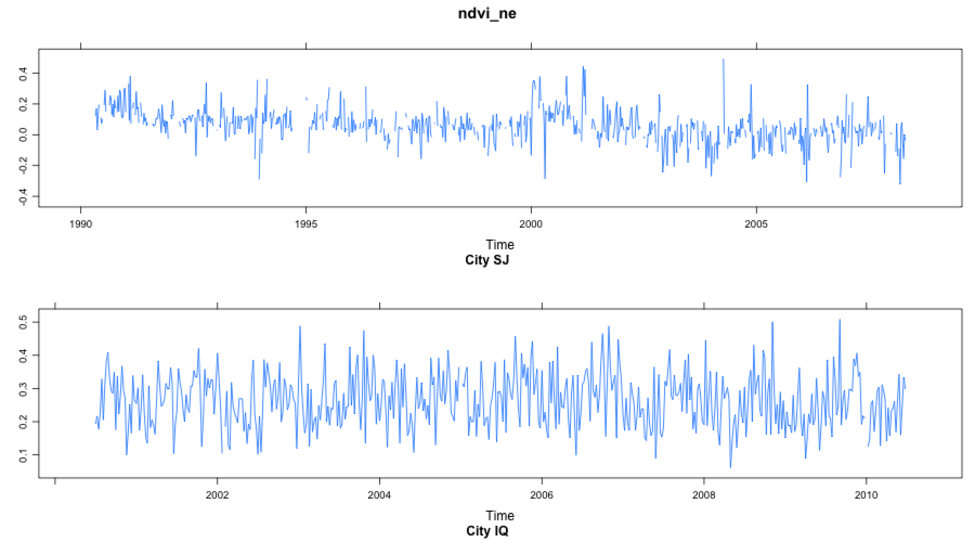
\includegraphics[width=\textwidth]{Final_report_files/figure-latex/unnamed-chunk-1-1} \caption{ }\label{fig:unnamed-chunk-1}
\end{figure}\begin{figure}[!h]
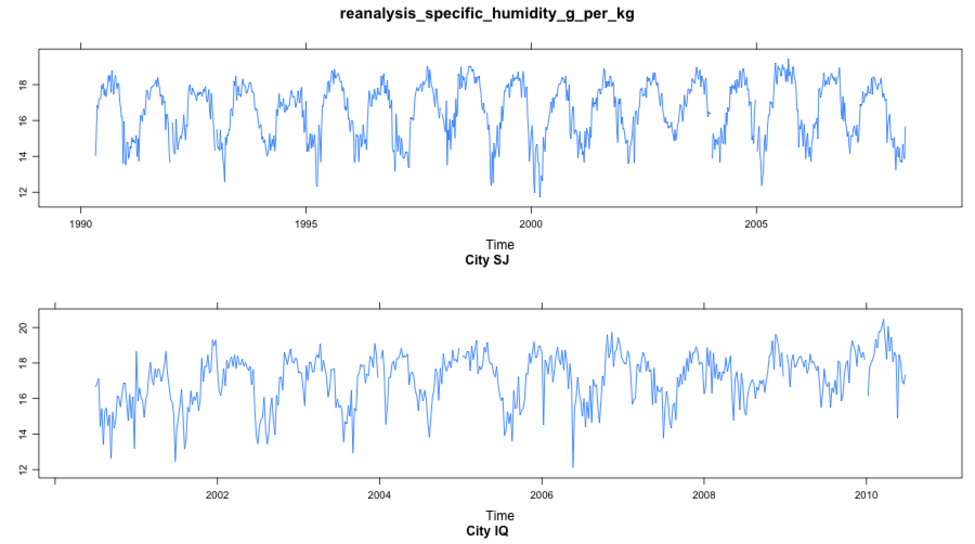
\includegraphics[width=\textwidth]{Final_report_files/figure-latex/unnamed-chunk-2-1} \caption{ }\label{fig:unnamed-chunk-2}
\end{figure}\begin{figure}[!h]
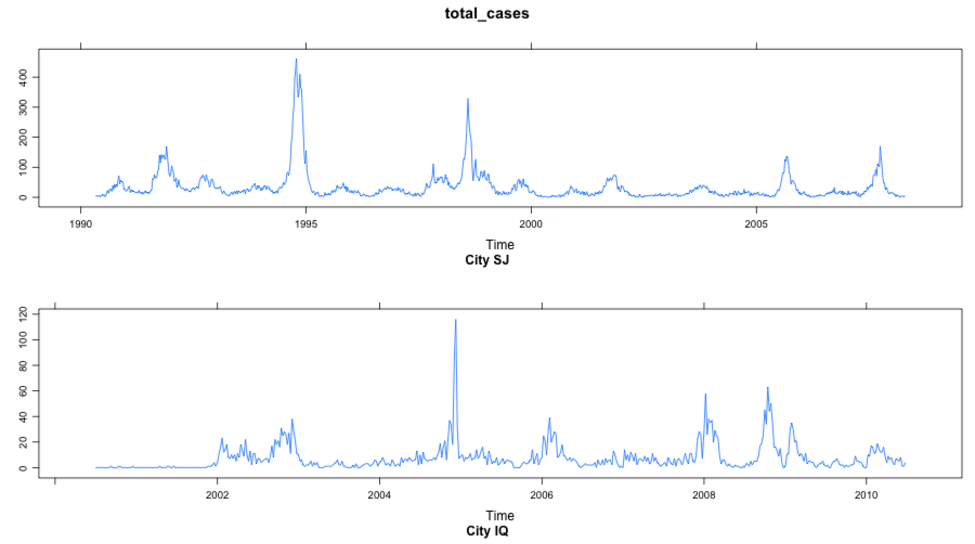
\includegraphics[width=\textwidth]{Final_report_files/figure-latex/unnamed-chunk-3-1} \caption{ }\label{fig:unnamed-chunk-3}
\end{figure}

\newpage

\begin{enumerate}
\def\labelenumi{\arabic{enumi}.}
\tightlist
\item
  Multivariate studies (Linear Correlations)
\end{enumerate}

Linear correlation study between the Xs and Y for the two cities show
remarkable difference between the cities, along with some key insights
into the underlying structure of the data. Some key highlights:

\begin{itemize}
\item
  \texttt{total\_cases} is very weakly correlated (if at all) with any
  of the Xs. Doesn't let itself to a simple way of predicting the
  values. It's weakly correlated with the \texttt{weekofyear} variable,
  which makes sense. When it's hotter, and wetter, there is a higher
  chance of dengue.
\item
  SJ's corrplot shows us that almost all the correlations are positive,
  it at all. As expected, all the vegetation indices are correlated
  positively. As are all the temperature related variables. Further
  investigation using PCA showed me that for these variable groups, at
  max 2 PCs were needed to achieve \textasciitilde{}97\%+ of explanatory
  power for the variation in each group.
\item
  IQ's corrplot has a few strong negative correlations, especially with
  the \texttt{tdtr} variable, which explains the daily temperature
  fluctuation. When it's very hot, or very humid, there is less
  temperature variable over the day. Given IQ's geographic location,
  perhaps this makes sense from a weather dynamics standpoint.
\end{itemize}

\begin{figure}[!h]
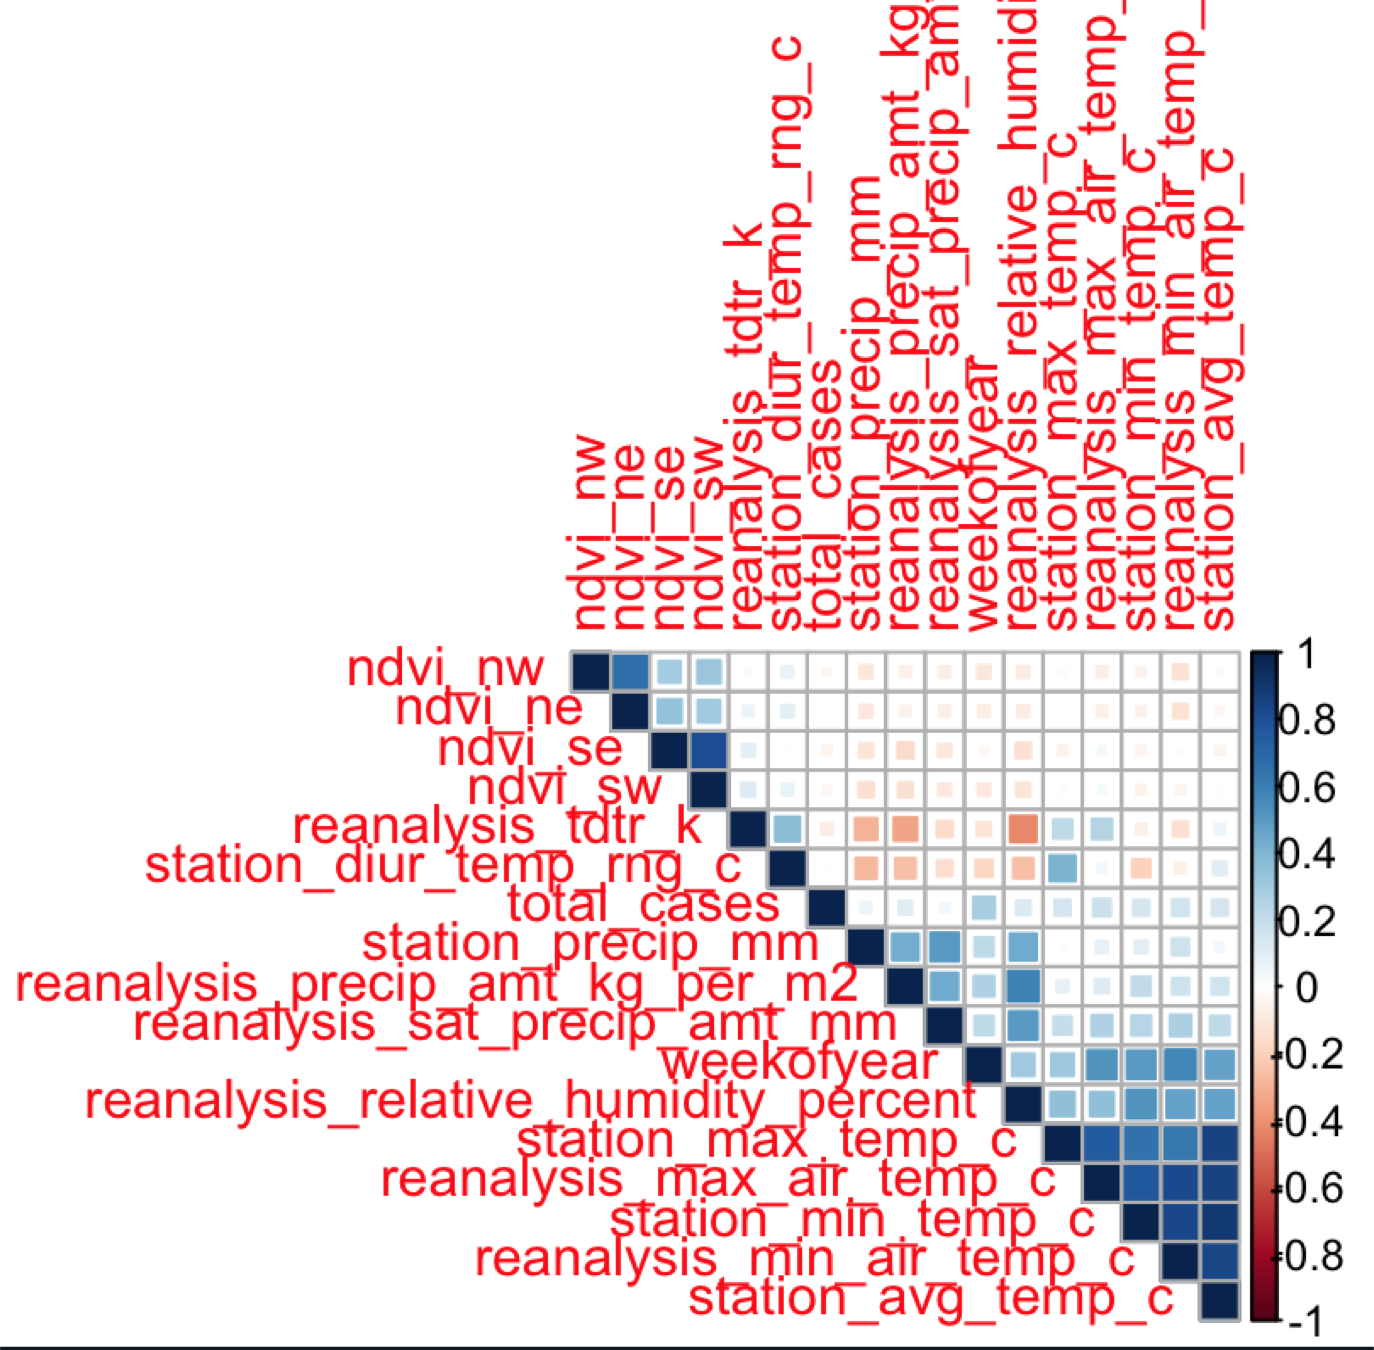
\includegraphics[width=0.5\linewidth]{Final_report_files/figure-latex/unnamed-chunk-4-1} \caption{ }\label{fig:unnamed-chunk-4}
\end{figure}\begin{figure}[!h]
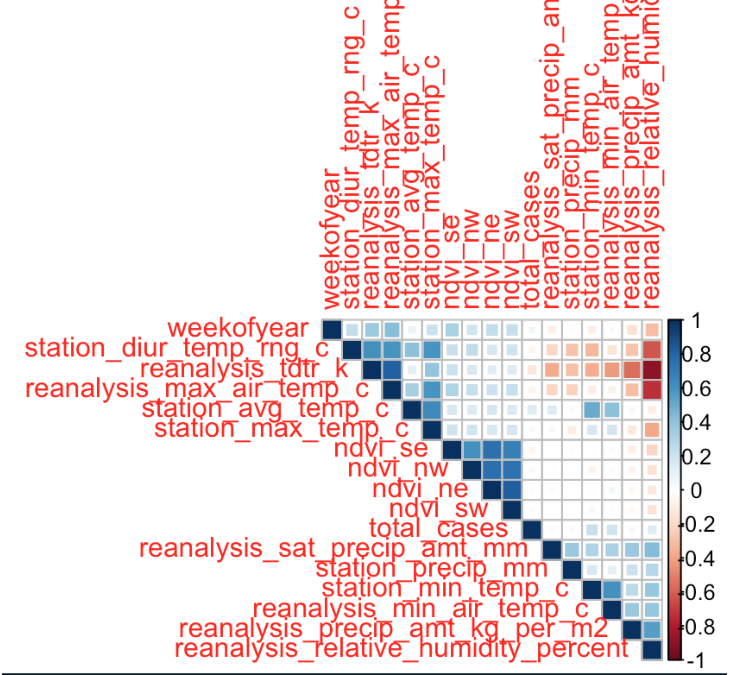
\includegraphics[width=\textwidth]{Final_report_files/figure-latex/unnamed-chunk-5-1} \caption{ }\label{fig:unnamed-chunk-5}
\end{figure}

\newpage

\section{Section III - Data
Preparation}\label{section-iii---data-preparation}

The summary of the data preparation activities is:

\begin{itemize}
\item
\end{itemize}

\subsubsection{Imputation}\label{imputation}

\subsubsection{Feature Engineering}\label{feature-engineering}

\newpage

\section{Section IV - Method of
Analogues}\label{section-iv---method-of-analogues}

\paragraph{Method Details}\label{method-details}

\paragraph{Transfer Entropy}\label{transfer-entropy}

\paragraph{Computational Details}\label{computational-details}

\paragraph{Internal Test Set}\label{internal-test-set}

\paragraph{Drivendata.org Test Set}\label{drivendata.org-test-set}

\newpage

\section{Section V - Deep Learning
Models}\label{section-v---deep-learning-models}

\subsubsection{GRU or LSTM graph tree}\label{gru-or-lstm-graph-tree}

\subsubsection{Hyperparameter tuning}\label{hyperparameter-tuning}

\subsubsection{Performance Evaluation}\label{performance-evaluation}

\paragraph{Internal Test Set}\label{internal-test-set-1}

\paragraph{Drivendata.org Test Set}\label{drivendata.org-test-set-1}

\section{Section VI - Bayesian Regression
Model}\label{section-vi---bayesian-regression-model}

\subsubsection{Few notes}\label{few-notes}

\section{Section VII - Wrap Up}\label{section-vii---wrap-up}

\begin{enumerate}
\def\labelenumi{\arabic{enumi}.}
\item
  The MOA model shows promise for one-step-ahead (or few-steps-ahead)
  forecasting, as long as there is enough history of the multivariate
  signals. Further investigation into methods of identification of
  analogues (PCA, Mahanobalis distance etc) might prove useful. Also,
  the search algorithm is expensive as implemented using for loops in R.
  Moving a lower level language like C++ might show execution speed
  improvements.
\item
\end{enumerate}

\newpage

\section{R Packages Used}\label{r-packages-used}

\newpage

\section{References}\label{references}

\begin{enumerate}
\def\labelenumi{\arabic{enumi}.}
\tightlist
\item
  Buczak, A. L., Baugher, B., Moniz, L. J., Bagley, T., Babin, S. M., \&
  Guven, E. (2018). Ensemble method for dengue prediction. PLoS ONE,
  13(1), e0189988. \url{http://doi.org/10.1371/journal.pone.0189988}
\item
  Vicente, R., Wibral, M., Lindner, M., \& Pipa, G. (2011). Transfer
  entropy---a model-free measure of effective connectivity for the
  neurosciences. Journal of Computational Neuroscience, 30(1), 45--67.
  \url{http://doi.org/10.1007/s10827-010-0262-3}
\item
  Viboud C, Boelle P-Y, Carrant F, Valleron A-J, Flahault A. Prediction
  of the spread of influenza epidemics by the Method of Analogues.
  American Journal of Epidemiology 2003; \url{http://10.1093/aje/kwg239}
\item
  Lorenz E. Atmospheric predictability as revealed by naturally
  occurring analogies. Journal of Atmospheric Science 1969; 26:636--646
  1.\url{https://github.com/amschwinn/dengue_prediction}
\item
  \url{https://cran.r-project.org/web/packages/TransferEntropy/TransferEntropy.pdf}
\item
  \url{https://ral.ucar.edu/sites/default/files/public/images/events/WISE_documentation_20170725_Final.pdf}
\item
  \url{https://tensorflow.rstudio.com/keras/}
\item
  \url{https://tensorflow.rstudio.com/blog/time-series-forecasting-with-recurrent-neural-networks.html}
\end{enumerate}

\begingroup
\setlength{\parindent}{-0.5in} \setlength{\leftskip}{0.5in}

\hypertarget{refs}{}

\endgroup






\end{document}
